\section{Half Body Error Estimation}
\label{sec:half_body}

The second model that was developed was the half body model. The half body model was trained to give two error labels as an output given an image as an input, one for the lower body and one for the upper body. The results of the training process of the Half Body model can be seen in Figure \ref{fig:half_body_training_results}.

\begin{figure}
  \centering
  \begin{subfigure}[b]{0.8\textwidth}
      \centering
      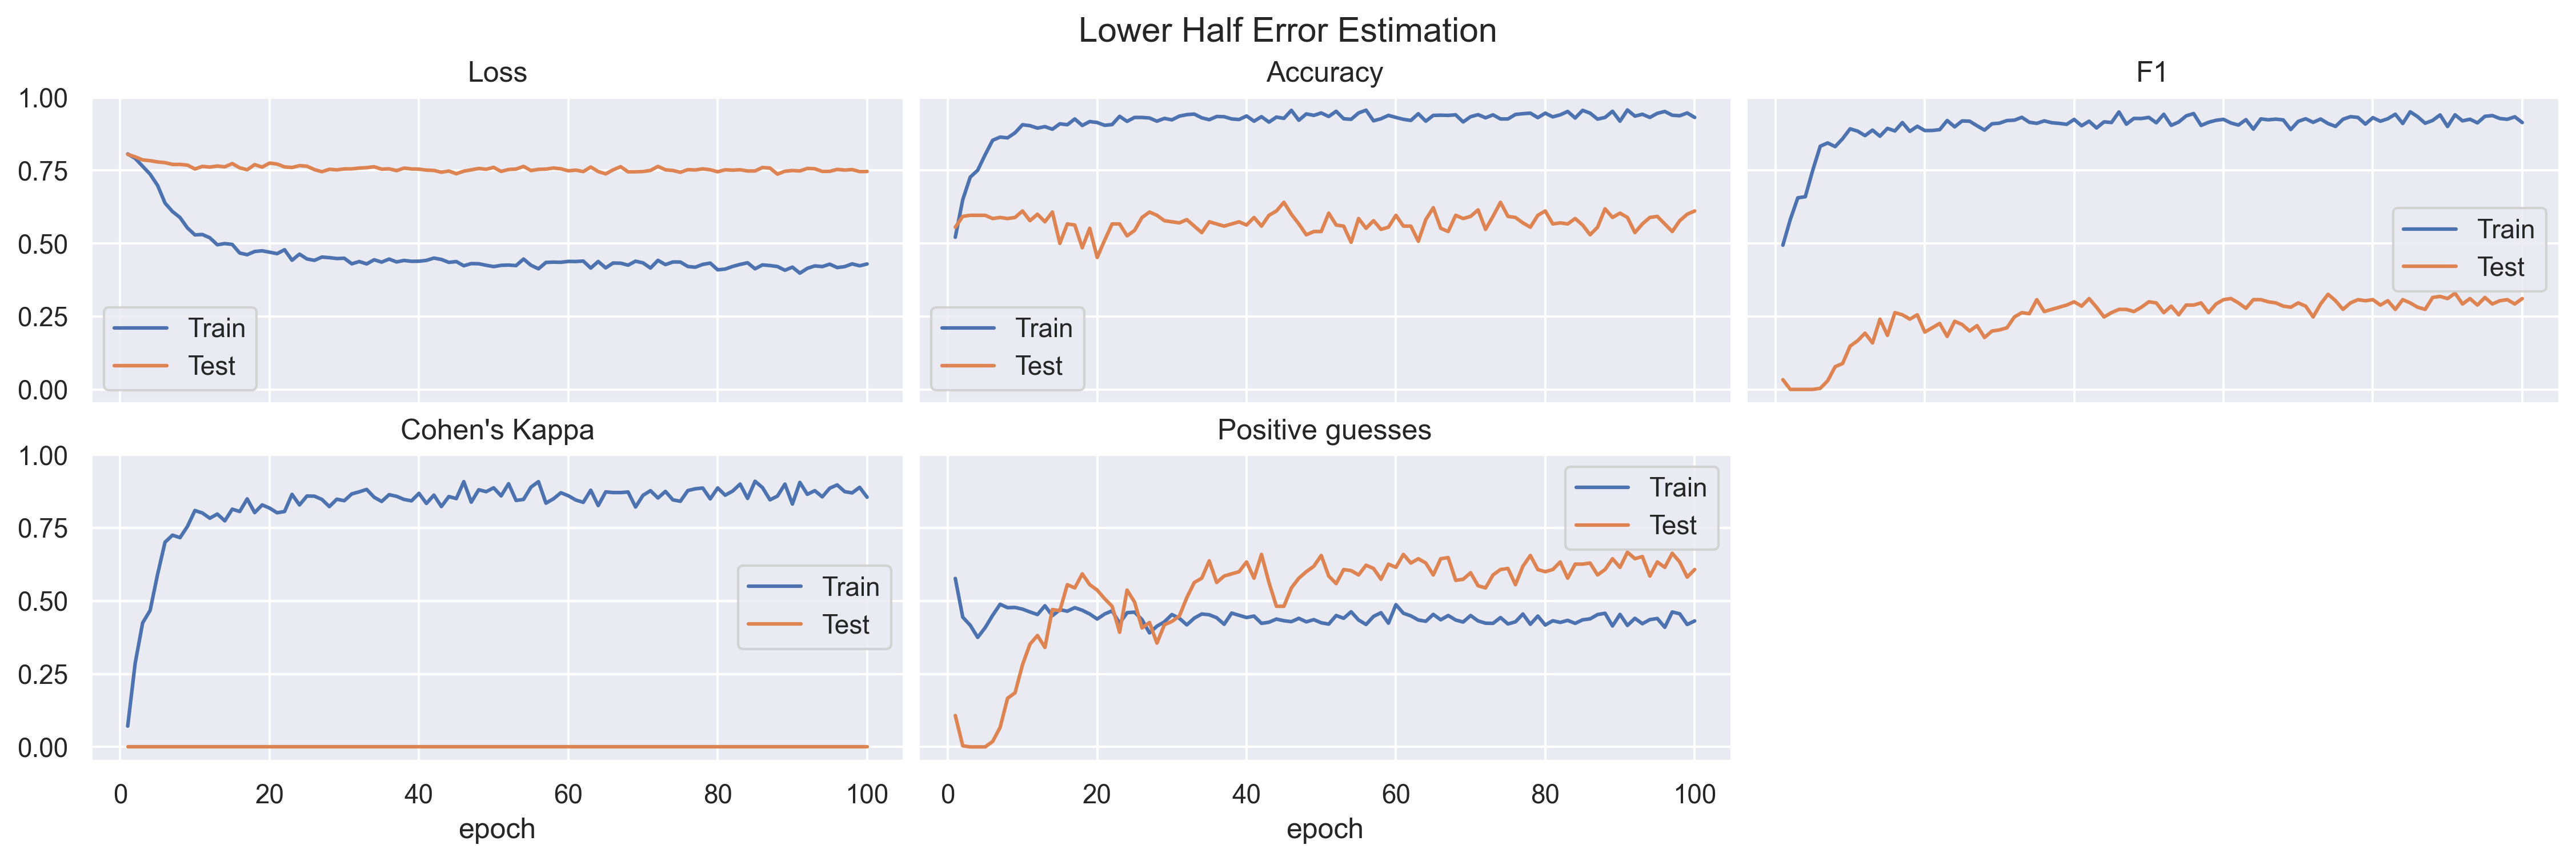
\includegraphics[width=\textwidth]{figures/Results/hb/HalfBodyErrorEstimation_uh.png}
      \caption{Upper Body Error Estimation}
      \label{fig:uh_ee}
  \end{subfigure}
  \hfill
  \begin{subfigure}[b]{0.8\textwidth}
      \centering
      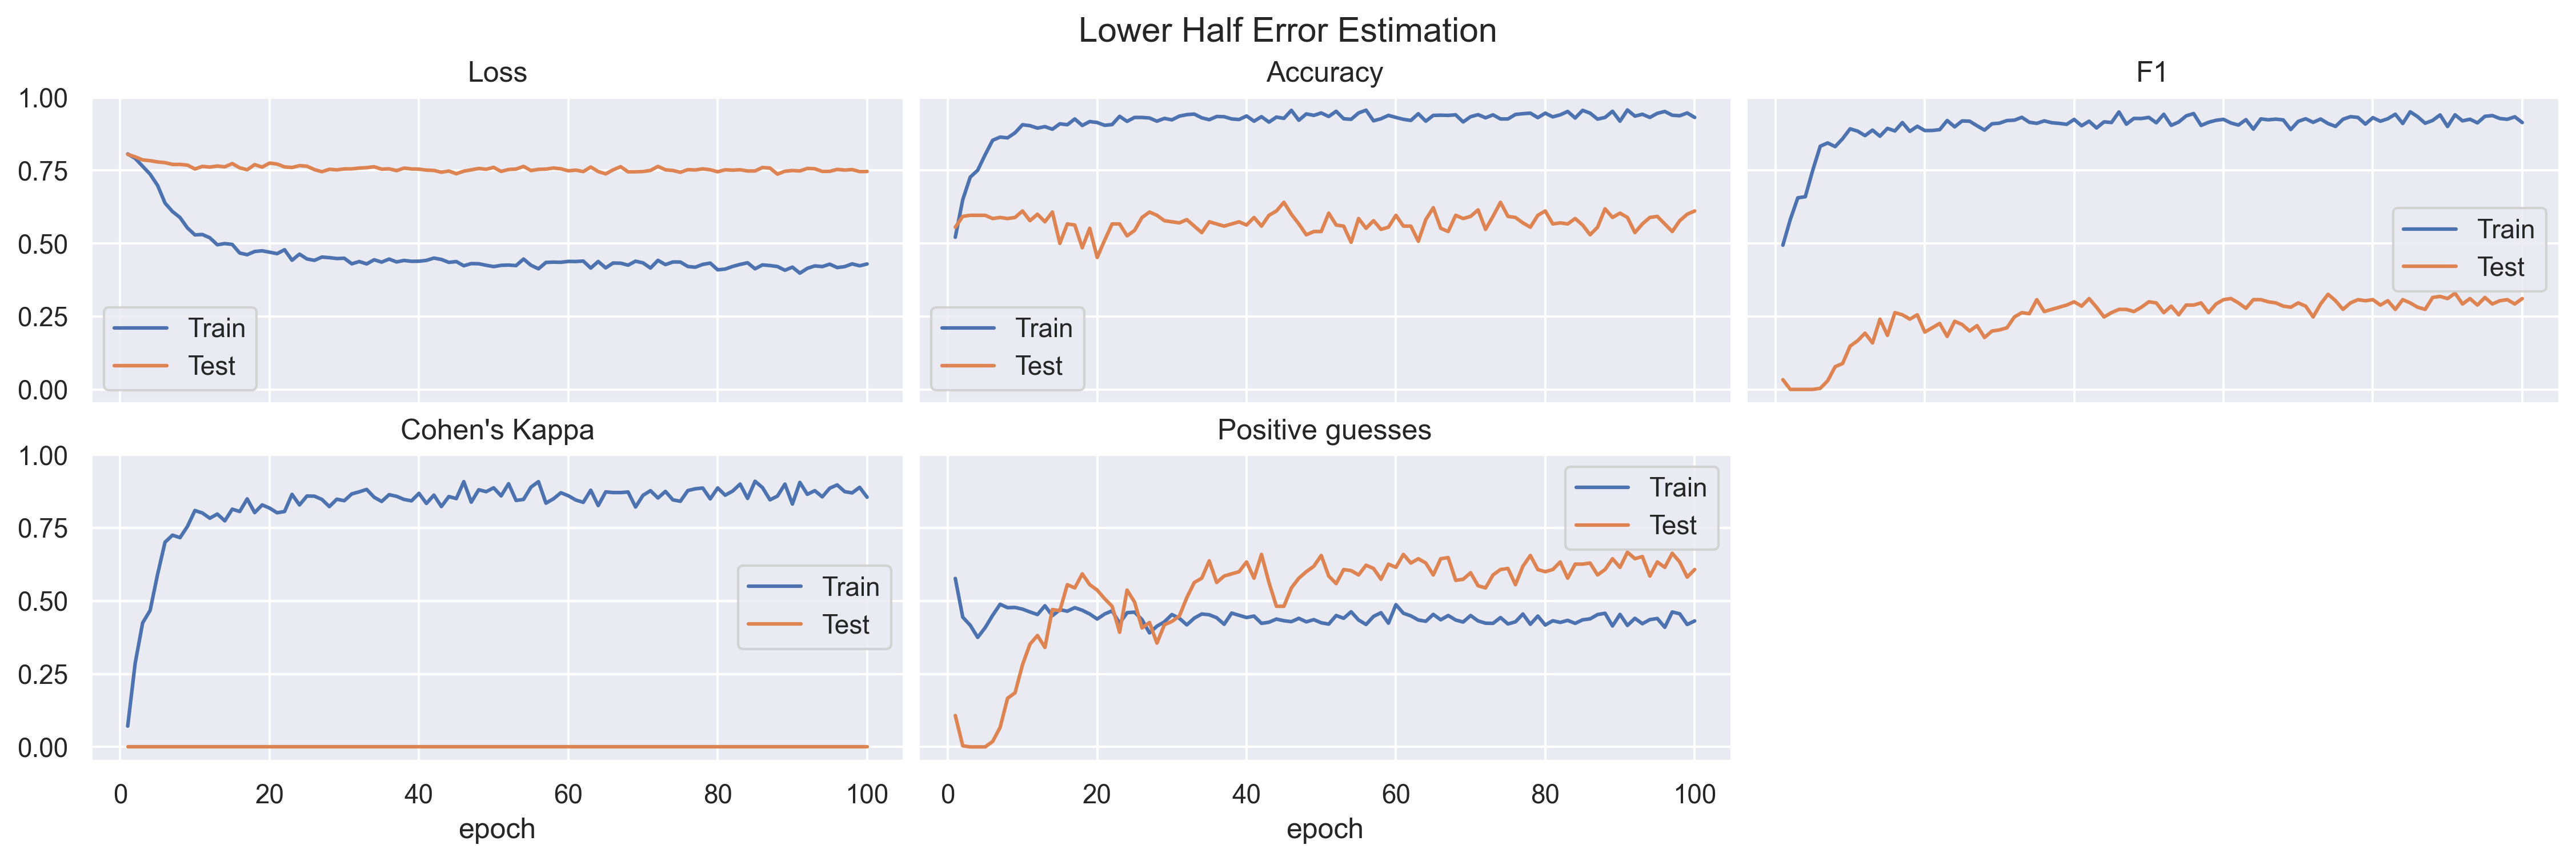
\includegraphics[width=\textwidth]{figures/Results/hb/HalfBodyErrorEstimation_lh.png}
      \caption{Lower Body Error Estimation}
      \label{fig:lh_ee}
  \end{subfigure}
  \caption[Half Body model training results]{The training results of the half body error estimation model.}
     \label{fig:half_body_training_results}
\end{figure}

\subsubsection{Confusion Matrix}

The confusion matrix of the half body model is shown in Figure \ref{fig:half_body_confusion_matrix}. It can be seen that contrary to the full body model the half body model variies the error label. 

\begin{figure}
  \centering
  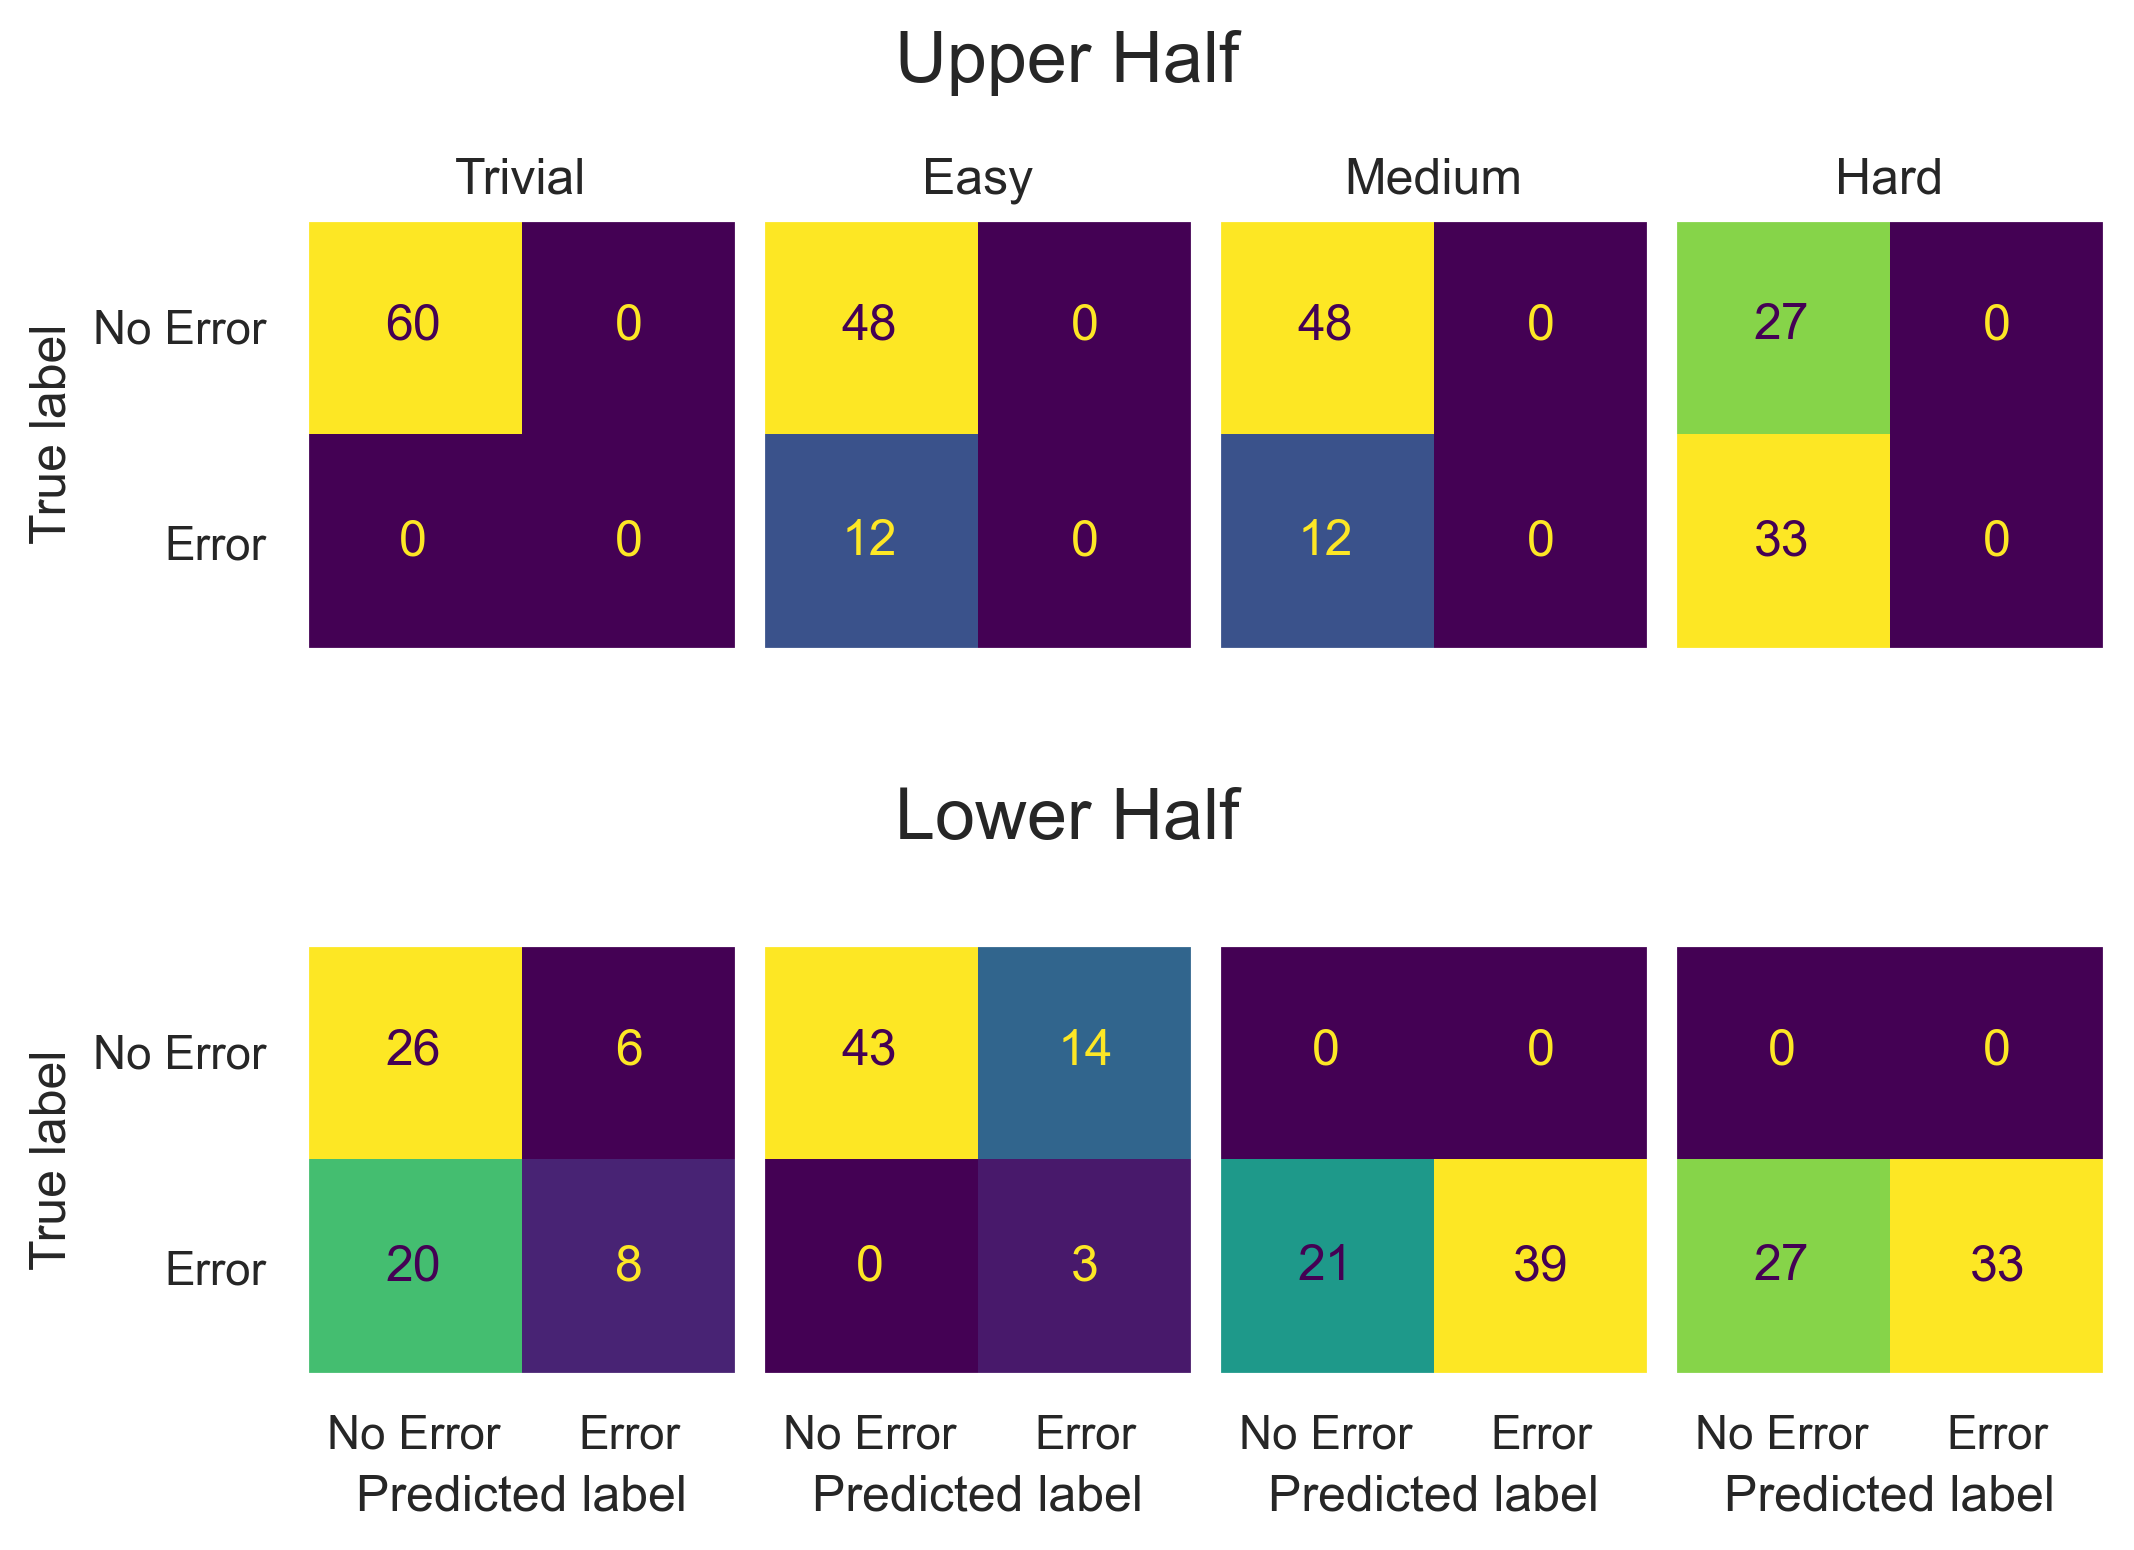
\includegraphics[width=0.8\textwidth]{figures/results/confusion/halves.png}
  \caption[Half Body model confusion matrix]{The confusion matrix of the half body model.}
  \label{fig:half_body_confusion_matrix}
\end{figure}

\subsection{Emulated Full Body}

The results of the model can be used to emulate the full body model. Therefore, the two models can be compared. The results of the model are shown in Figure \ref{fig:half_body_emulated_full_body}. It can be seen that the half body model outperforms the full body model. The reason for this is that the full body model estimates purely positive results, whereas the half body models variies as is shown in the ${p}\over{p+n}$ graph, which shows the percentage of positive guesses.

\begin{figure}
  \centering
  %\includegraphics[width=0.8\textwidth]{figures/results/Half_Body/Emulated_Full_Body.png}
  \caption[Half Body model with emulated Full Body results]{The results of the half body model when emulating the full body results.}
  \label{fig:half_body_emulated_full_body}
\end{figure}
